The graphs printed during training (the notebooks' \texttt{plot\_training}, \texttt{plot\_metrics} and
\texttt{plot\_robustness\_curves}) for every 15k-step, seed-0 run of Table~\ref{tab:h1} and the context-noise run of
Sec.~\ref{sec:noise}, one curve per run in every panel. The evaluation curves use the fixed probe setting
(lr $3{\cdot}10^{-3}$, wd $10^{-4}$) every 50 steps, so they are descriptive only; the reported numbers use the
validation-selected probe. Step 0 is the random initialisation.

\begin{figure}[!ht]
\centering
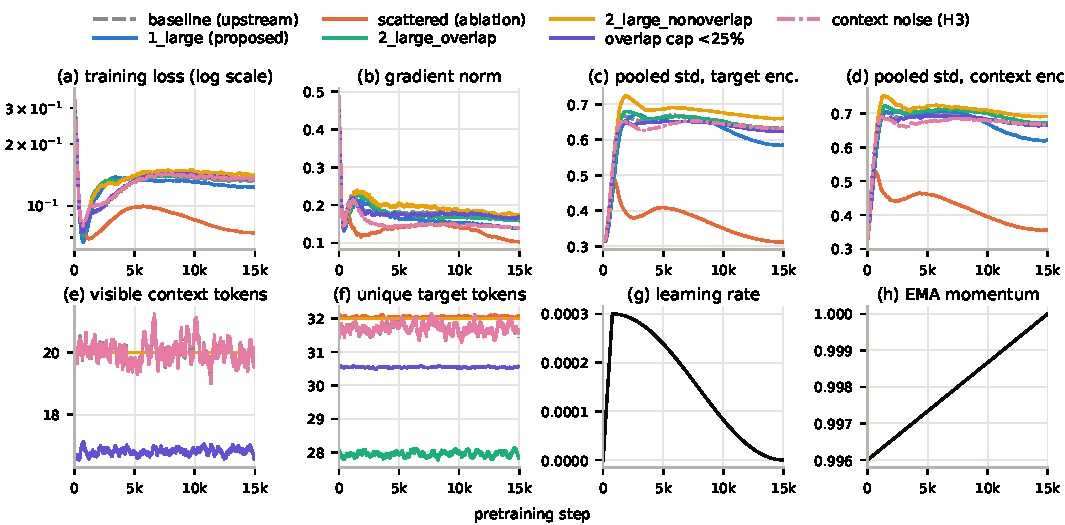
\includegraphics[width=\linewidth]{figures/fig_app_training.pdf}
\caption{Training signals, logged every step (moving average over 300 steps). (c)--(d) std over the batch of the
mean-pooled tokens, averaged over the 128 dimensions; (d) for context noise is measured on the noised context input.
(e) context tokens after the batch-minimum trim; (f) distinct target patches per image (a patch covered by two blocks
counts once). Baseline and context noise use identical masks, so their curves coincide in (e)--(f).
(g)--(h) the same schedule for every run. The per-block runs (scattered, 2\_large, overlap cap)
were trained before (b)--(d) and (f) were logged; their curves come from a retraining with the same seed and config.}
\label{fig:app_training}
\end{figure}

\begin{figure}[!ht]
\centering
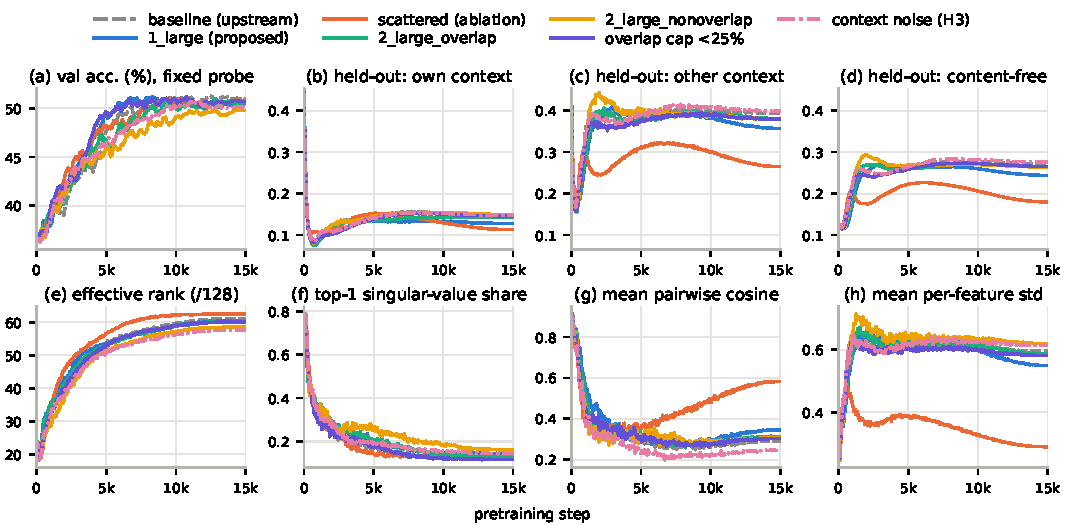
\includegraphics[width=\linewidth]{figures/fig_app_metrics.pdf}
\caption{Periodic evaluation (every 50 steps). (a) validation accuracy of the fixed probe (moving average over 5
evaluations). (b)--(d) held-out latent loss (``held-out'') on the validation images with fixed upstream masks (seed 12345): with the
image's own context, with another image's context, and for the content-free per-position mean target; the three
panels share one y-range. (e)--(h) collapse statistics of the pooled clean test features.}
\label{fig:app_metrics}
\end{figure}

\begin{figure}[!ht]
\centering
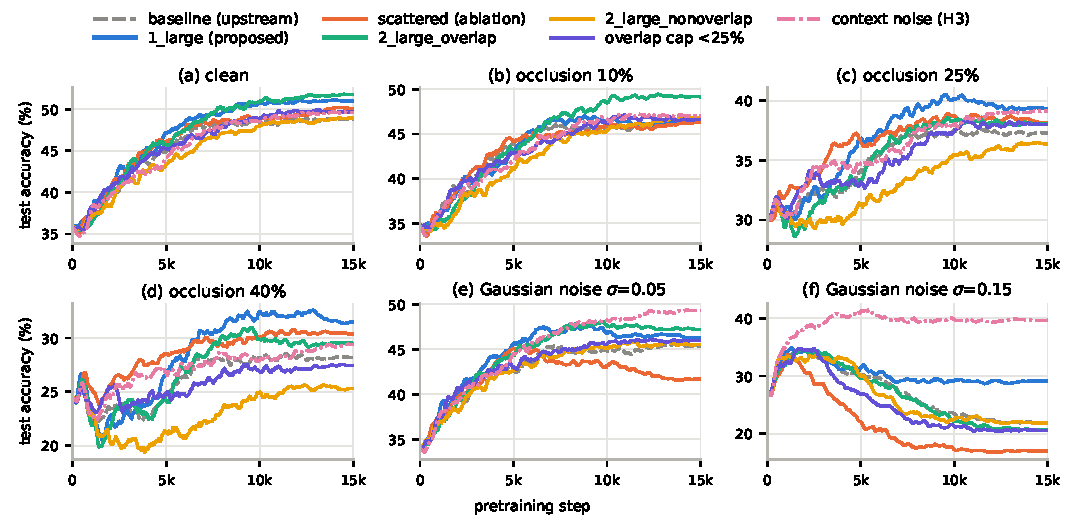
\includegraphics[width=\linewidth]{figures/fig_app_robustness.pdf}
\caption{Test accuracy per condition with the fixed clean-trained probe (moving average over 5 evaluations; chance is 10\%). Descriptive only, never used for selection.}
\label{fig:app_robustness}
\end{figure}
